% !TEX program = xelatex
% Bo slide thuyet trinh 7 slide -- SoICT HUST Summer School 2026 (Edge AI)
\documentclass[aspectratio=169]{beamer}

\usetheme{Madrid}
\usefonttheme{professionalfonts}

\usepackage{fontspec}
\setmainfont{Arial}
\setmonofont{Consolas}

\usepackage{tikz}
\usetikzlibrary{arrows.meta,positioning,fit,backgrounds,shapes.geometric,calc,shadows.blur}
\usepackage{booktabs}
\usepackage{listings}
\usepackage{xcolor}
\usepackage{hyperref}
\usepackage{fontawesome5}
\usepackage{graphicx}

% ---------------------------------------------------------------------------
% Bang mau lay tu giao dien web tren box (server.py)
% ---------------------------------------------------------------------------
\definecolor{oeNavy}{HTML}{0B2136}
\definecolor{oeBlue}{HTML}{1F6F91}
\definecolor{oeSky}{HTML}{2A8FC0}
\definecolor{oeGreen}{HTML}{1FA97A}
\definecolor{oeRed}{HTML}{C0453F}
\definecolor{oeLightBg}{HTML}{F3F7FA}
\definecolor{oeGray}{HTML}{5B6B7C}
\definecolor{hustRed}{HTML}{A6192E}
\definecolor{hustGold}{HTML}{F0B429}

\setbeamercolor{structure}{fg=oeNavy}
\setbeamercolor{palette primary}{bg=oeNavy,fg=white}
\setbeamercolor{palette secondary}{bg=oeBlue,fg=white}
\setbeamercolor{palette tertiary}{bg=oeNavy,fg=white}
\setbeamercolor{palette quaternary}{bg=oeNavy,fg=white}
\setbeamercolor{title}{fg=white}
\setbeamercolor{subtitle}{fg=white}
\setbeamercolor{author}{fg=oeNavy}
\setbeamercolor{institute}{fg=oeGray}
\setbeamercolor{date}{fg=oeGray}
\setbeamercolor{frametitle}{bg=oeNavy,fg=white}
\setbeamercolor{block title}{bg=oeBlue,fg=white}
\setbeamercolor{block body}{bg=oeLightBg,fg=oeNavy}
\setbeamercolor{block title alerted}{bg=oeRed,fg=white}
\setbeamercolor{block body alerted}{bg=oeLightBg,fg=oeNavy}
\setbeamercolor{itemize item}{fg=oeGreen}
\setbeamercolor{itemize subitem}{fg=oeSky}
\setbeamertemplate{navigation symbols}{}
\setbeamertemplate{headline}{}
\setbeamertemplate{itemize item}{\raise1pt\hbox{\textbullet}}

\setbeamertemplate{footline}{%
  \begin{beamercolorbox}[wd=\paperwidth,ht=3.0ex,dp=1.4ex,leftskip=3mm,rightskip=3mm]{page number in head/foot}
    
\includegraphics[height=1.9ex]{assets/soict_hust_logo.png}\hspace{5pt}%
    {\tiny\color{oeGray} SoICT Summer School 2026 -- Edge AI}%
    \hfill{\tiny\color{oeGray} OmniGlass Edge}\hfill%
    {\tiny\color{oeGray}\insertframenumber{}/\inserttotalframenumber}
  \end{beamercolorbox}
}

\lstset{
  basicstyle=\ttfamily\scriptsize\color{oeNavy},
  breaklines=true,
  columns=fullflexible,
  backgroundcolor=\color{oeLightBg},
  frame=single,
  rulecolor=\color{oeGray},
  framerule=0.3pt,
  xleftmargin=4pt,
  xrightmargin=4pt
}

\title{OmniGlass Edge}
\subtitle{\small Trợ lý đa phương thức Edge AI cho người khiếm thị -- chạy hoàn toàn on-device trên Qualcomm QCS8550}
\author{Nhóm 2}
\institute{\small SoICT HUST Summer School 2026 -- Trí tuệ nhân tạo tại biên (Edge AI)}
\date{\small Báo cáo Project, 10--14/08/2026}
\titlegraphic{
\includegraphics[width=3.6cm]{assets/soict_hust_logo.png}}

\begin{document}

% =============================================================================
\begin{frame}
  \titlepage
\end{frame}

% =============================================================================
\begin{frame}{Động lực: vì sao phải là Edge, không phải Cloud?}
  \begin{columns}[T]
    \begin{column}{0.44\textwidth}
      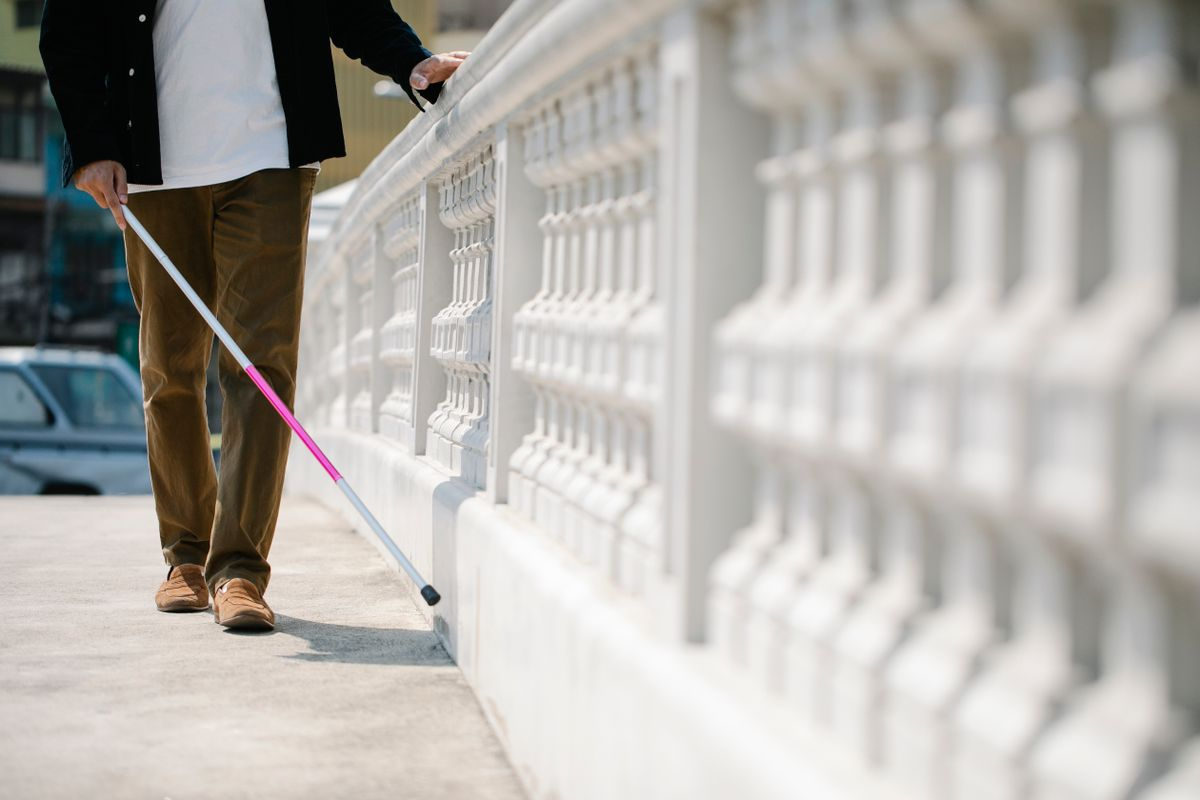
\includegraphics[width=\linewidth]{assets/motivation_photo.jpg}
      \vspace{2pt}
      {\tiny\color{oeGray} Ảnh minh họa: người khiếm thị di chuyển bằng gậy dò đường (Pexels, free license).}
    \end{column}
    \begin{column}{0.56\textwidth}
      \begin{itemize}
        \item Người khiếm thị cần \textbf{nhận biết môi trường} và \textbf{giao tiếp
              rảnh tay theo thời gian thực} -- một trợ lý cảnh báo nguy hiểm không
              được phép trễ hay mất kết nối.
        \item \textbf{Cloud VLM}: round-trip 100s\,ms--vài giây, cần mạng liên tục,
              camera/mic phải rời khỏi thiết bị -- rủi ro cho một use-case an toàn.
        \item \textbf{OmniGlass Edge}: detect + depth + STT + VLM + TTS chạy
              \textbf{cục bộ 100\%} trên một board Qualcomm QCS8550 duy nhất --
              không phải demo model trên laptop rồi gọi là ``edge''.
      \end{itemize}
    \end{column}
  \end{columns}
\end{frame}

% =============================================================================
\begin{frame}{Quy trình phát triển Edge AI: Model $\to$ Convert/Optimize $\to$ Deploy $\to$ App}
  \centering
  \begin{tikzpicture}[
      font=\scriptsize,
      node distance=4mm,
      stage/.style={draw=oeBlue, fill=oeLightBg, rounded corners=3pt, text width=2.75cm,
                    align=left, minimum height=3.1cm, thick,
                    blur shadow={shadow blur steps=6, shadow xshift=0.4pt,
                                 shadow yshift=-1.2pt, shadow blur radius=2pt}},
      arr/.style={-{Latex[length=2.5mm]}, thick, oeGray}
    ]
    \node[stage] (m1) {
      \centering\faBrain\ \textbf{1. Model}\\[3pt]
      \raggedright\footnotesize
      YOLO11 (detect)\\ Depth (mono)\\ Whisper (STT)\\ Qwen3.5 2B VL\\ VieNeu (TTS)
    };
    \node[stage, right=of m1] (m2) {
      \centering\faSlidersH\ \textbf{2. Convert /}\\\textbf{Optimize}\\[3pt]
      \raggedright\footnotesize
      Whisper Small$\to$Base Q8\\ Silero VAD ctx-512\\ Detect/depth $\to$ QNN\\ Bench CPU/GPU/NPU
    };
    \node[stage, right=of m2] (m3) {
      \centering\faRocket\ \textbf{3. Deploy}\\[3pt]
      \raggedright\footnotesize
      whisper.cpp build\\ARM NEON tại target\\ Push qua ADB\\
      \texttt{/data/local/tmp}\\ Service Python + JSON config
    };
    \node[stage, right=of m3] (m4) {
      \centering\faDesktop\ \textbf{4. Application}\\[3pt]
      \raggedright\footnotesize
      Web UI push-to-talk\\ Camera MJPEG stream\\ TTS streaming ra loa\\
      Orchestrator hợp nhất pipeline
    };
    \draw[arr] (m1) -- (m2);
    \draw[arr] (m2) -- (m3);
    \draw[arr] (m3) -- (m4);
  \end{tikzpicture}
  \vspace{6pt}

  {\scriptsize\color{oeGray} Mỗi mũi tên là một quyết định kỹ thuật thật đã đưa ra
  và đo lại bằng benchmark trên chính board QCS8550 -- không chỉ là sơ đồ lý thuyết.}
\end{frame}

% =============================================================================
\begin{frame}[fragile]{Kiến trúc runtime trên thiết bị (đang chạy thật)}
  \centering
  \begin{tikzpicture}[
      font=\scriptsize,
      node distance=6mm,
      box/.style={draw=oeBlue, fill=oeLightBg, rounded corners=2pt, text width=2.0cm,
                  align=center, minimum height=1.05cm, thick,
                  blur shadow={shadow blur steps=6, shadow xshift=0.4pt,
                               shadow yshift=-1.2pt, shadow blur radius=2pt}},
      always/.style={box, draw=oeGreen},
      talk/.style={box, draw=oeSky},
      arr/.style={-{Latex[length=2mm]}, thick, oeGray}
    ]
    \node[always] (cam) {\faCamera\\Camera\\\texttt{/dev/video2}};
    \node[always, right=of cam] (yolo) {\faCrosshairs\\YOLO11\\detect+depth};
    \node[always, right=of yolo] (htp) {\faMicrochip\\Hexagon HTP\\(QNN)};
    \node[right=of htp, text width=2.2cm, align=center, font=\scriptsize\bfseries, color=oeGreen]
      (loopnote) {Always-on\\$\approx$23--24 FPS};

    \draw[arr] (cam) -- (yolo);
    \draw[arr] (yolo) -- (htp);
    \draw[arr] (htp) -- (loopnote);

    \node[talk, below=13mm of cam] (mic) {\faMicrophone\\Push-to-talk\\mic};
    \node[talk, right=of mic] (stt) {\faClosedCaptioning\\Whisper STT\\CPU NEON};
    \node[talk, right=of stt] (vlm) {\faRobot\\Qwen3.5 2B VL\\llama.cpp};
    \node[talk, right=of vlm] (tts) {\faWaveSquare\\VieNeu TTS\\stream PCM};
    \node[talk, right=of tts] (spk) {\faVolumeUp\\Speaker\\ALSA/PC};

    \draw[arr] (mic) -- (stt);
    \draw[arr] (stt) -- (vlm);
    \draw[arr] (vlm) -- (tts);
    \draw[arr] (tts) -- (spk);
    \draw[arr, dashed] (htp.south) |- ($(vlm.north)+(0,4mm)$) -- (vlm.north);
  \end{tikzpicture}

  \vspace{4pt}
  \begin{lstlisting}
"scene": {"camera_ok": true, "depth_ok": true, "frame_age_ms": 9.5}
"resources": {"detector_fps": 23.40, "npu_temperature_c": 80.8}
\end{lstlisting}
  {\scriptsize\color{oeGray} Telemetry đọc trực tiếp từ \texttt{GET /health} trên box -- không phải số liệu dựng.}
\end{frame}

% =============================================================================
\begin{frame}{Bài toán kỹ thuật khó nhất: đưa STT lên biên an toàn}
  \centering
  \footnotesize
  \begin{tabular}{p{2.9cm}p{5.4cm}p{2.6cm}}
    \toprule
    \textbf{Hướng thử} & \textbf{Kết quả} & \textbf{Quyết định} \\
    \midrule
    GPU Adreno 740 (OpenCL) & Cả Q8 và FP16 đều \texttt{segfault} (exit 139) &
      \textcolor{oeRed}{\faTimesCircle\ Loại bỏ} \\
    NPU Hexagon HTP (QNN) & Cần QNN context export qua AI Hub -- chưa có credential &
      \textcolor{oeBlue}{\faClock\ Tương lai} \\
    Streaming thô (1,5\,s/chunk) & Tự sinh câu giả khi im lặng, mỗi chunk mất 2,7\,s &
      \textcolor{oeRed}{\faTimesCircle\ Loại bỏ} \\
    \textbf{CPU NEON, Base Q8 + VAD} & \textbf{8,75\,s audio $\to$ 2,48\,s (RTF 0,28)} &
      \textcolor{oeGreen}{\faCheckCircle\ Bản chính} \\
    \bottomrule
  \end{tabular}
  \vspace{6pt}
  \begin{alertblock}{Kết quả đo thực tế trên board}
    \footnotesize
    Detector \textbf{23,4--23,7 FPS} liên tục $\cdot$ STT RTF \textbf{0,28} $\cdot$
    TTS streaming 48\,kHz/1,5$\times$ $\cdot$ NPU admission gate tại \textbf{75$^\circ$C}
    (quan sát thực tế 79--83$^\circ$C).
  \end{alertblock}
\end{frame}

% =============================================================================
\begin{frame}{Demo trực tiếp \& an toàn: NPU chia sẻ, perception không bao giờ nhường}
  \begin{columns}[T]
    \begin{column}{0.52\textwidth}
      \textbf{\faPlayCircle\ Demo trực tiếp -- \url{http://localhost:8090}}
      \begin{itemize}
        \item Camera stream thật + nút giữ-để-nói (push-to-talk)
        \item Bảng thời gian từng lượt: STT, VLM first-token, chờ nhiệt, TTS
        \item Có \textbf{video demo dự phòng} kèm hồ sơ nộp, phòng rủi ro khi
              trình diễn trực tiếp
      \end{itemize}
    \end{column}
    \begin{column}{0.48\textwidth}
      \textbf{\faThermometerHalf\ Thermal Admission Guard}
      \begin{itemize}
        \item VLM chỉ được chạy khi NPU $\le 75^\circ$C
        \item Perception (YOLO/depth) và STT/TTS \textbf{không} bị chặn --
              hazard detection không bao giờ đứng chờ VLM
        \item Khi box nóng: câu hỏi xếp hàng, camera vẫn cảnh báo nguy hiểm
              liên tục
      \end{itemize}
    \end{column}
  \end{columns}
\end{frame}

% =============================================================================
\begin{frame}{Nộp sản phẩm \& Kết luận}
  \begin{block}{Yêu cầu nộp}
    \begin{itemize}
      \item \textcolor{oeGreen}{\faCheckCircle} \textbf{Source code} --
            \href{https://github.com/technoob05/omniglass-vietnamese-edge-ai}{\faGithub\ \texttt{github.com/technoob05/omniglass-vietnamese-edge-ai}} (public)
      \item \textcolor{oeBlue}{\faClock} \textbf{Video demo} -- quay trước buổi báo cáo, đính kèm cùng hồ sơ Drive
      \item \textcolor{oeGreen}{\faCheckCircle} \textbf{Slide trình bày} -- tài liệu này
    \end{itemize}
  \end{block}
  \vspace{6pt}
  \begin{itemize}
    \item Toàn bộ pipeline nhận thức + ngôn ngữ + giọng nói chạy \textbf{thật} trên
          board Qualcomm QCS8550, không phải mô phỏng.
    \item Mọi số liệu trong slide đều lấy từ \texttt{/health} thật hoặc test pass
          thật trên thiết bị.
    \item An toàn được thiết kế vào kiến trúc: một hướng streaming STT
          nhanh-nhưng-sai đã bị loại bỏ có chủ đích để bảo vệ vòng lặp cảnh báo
          nguy hiểm.
  \end{itemize}
  \vspace{8pt}
  \centering
  \Large\textbf{Cảm ơn -- Q\&A}
\end{frame}

\end{document}
